\hypertarget{group__linop__class}{}\section{Linop\+\_\+class}
\label{group__linop__class}\index{Linop\+\_\+class@{Linop\+\_\+class}}


The linear operator (\hyperlink{classgko_1_1LinOp}{Lin\+Op}) is a base class for all linear algebra objects in Ginkgo.  


Collaboration diagram for Linop\+\_\+class\+:
\nopagebreak
\begin{figure}[H]
\begin{center}
\leavevmode
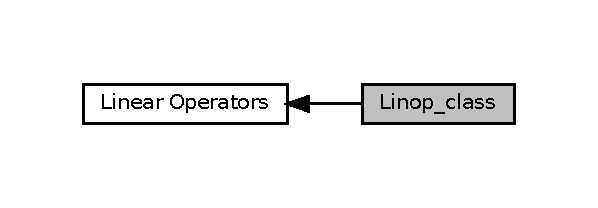
\includegraphics[width=287pt]{group__linop__class}
\end{center}
\end{figure}
The linear operator (\hyperlink{classgko_1_1LinOp}{Lin\+Op}) is a base class for all linear algebra objects in Ginkgo. 

The main benefit of having a single base class for the entire collection of linear algebra objects (as opposed to having separate hierarchies for matrices, solvers and preconditioners) is the generality it provides.

First, since all subclasses provide a common interface, the library users are exposed to a smaller set of routines. For example, a matrix-\/vector product, a preconditioner application, or even a system solve are just different terms given to the operation of applying a certain linear operator to a vector. As such, Ginkgo uses the same routine name, \hyperlink{classgko_1_1LinOp_a0449b2fc705d2f970855af23b5e2788e}{Lin\+Op\+::apply()} for each of these operations, where the actual operation performed depends on the type of linear operator involved in the operation.

Second, a common interface often allows for writing more generic code. If a user\textquotesingle{}s routine requires only operations provided by the \hyperlink{classgko_1_1LinOp}{Lin\+Op} interface, the same code can be used for any kind of linear operators, independent of whether these are matrices, solvers or preconditioners. This feature is also extensively used in Ginkgo itself. For example, a preconditioner used inside a Krylov solver is a \hyperlink{classgko_1_1LinOp}{Lin\+Op}. This allows the user to supply a wide variety of preconditioners\+: either the ones which were designed to be used in this scenario (like I\+LU or block-\/\+Jacobi), a user-\/supplied matrix which is known to be a good preconditioner for the specific problem, or even another solver (e.\+g., if constructing a flexible G\+M\+R\+ES solver).

A key observation for providing a unified interface for matrices, solvers, and preconditioners is that the most common operation performed on all of them can be expressed as an application of a linear operator to a vector\+:


\begin{DoxyItemize}
\item the sparse matrix-\/vector product with a matrix $A$ is a linear operator application $y = Ax$;
\item the application of a preconditioner is a linear operator application $y = M^{-1}x$, where $M$ is an approximation of the original system matrix $A$ (thus a preconditioner represents an \char`\"{}approximate
    inverse\char`\"{} operator $M^{-1}$).
\item the system solve $Ax = b$ can be viewed as linear operator application $x = A^{-1}b$ (it goes without saying that the implementation of linear system solves does not follow this conceptual idea), so a linear system solver can be viewed as a representation of the operator $A^{-1}$.
\end{DoxyItemize}

Finally, direct manipulation of \hyperlink{classgko_1_1LinOp}{Lin\+Op} objects is rarely required in simple scenarios. As an illustrative example, one could construct a fixed-\/point iteration routine $x_{k+1} = Lx_k + b$ as follows\+:


\begin{DoxyCode}
std::unique\_ptr<matrix::Dense<>> calculate\_fixed\_point(
        \textcolor{keywordtype}{int} iters, \textcolor{keyword}{const} LinOp *L, \textcolor{keyword}{const} matrix::Dense<> *x0
        \textcolor{keyword}{const} matrix::Dense<> *b)
\{
    \textcolor{keyword}{auto} x = gko::clone(x0);
    \textcolor{keyword}{auto} tmp = gko::clone(x0);
    \textcolor{keyword}{auto} \hyperlink{namespacegko_a0059e27f8f4bc348ff65c1e60caf47c8}{one} = Dense<>::create(L->get\_executor(), \{1.0,\});
    \textcolor{keywordflow}{for} (\textcolor{keywordtype}{int} i = 0; i < iters; ++i) \{
        L->apply(gko::lend(tmp), gko::lend(x));
        x->add\_scaled(gko::lend(\hyperlink{namespacegko_a0059e27f8f4bc348ff65c1e60caf47c8}{one}), gko::lend(b));
        tmp->copy\_from(gko::lend(x));
    \}
    \textcolor{keywordflow}{return} x;
\}
\end{DoxyCode}


Here, if $L$ is a matrix, \hyperlink{classgko_1_1LinOp_a0449b2fc705d2f970855af23b5e2788e}{Lin\+Op\+::apply()} refers to the matrix vector product, and {\ttfamily L-\/$>$apply(a, b)} computes $b = L \cdot a$. {\ttfamily x-\/$>$add\+\_\+scaled(one.\+get(), b.\+get())} is the {\ttfamily axpy} vector update $x:=x+b$.

The interesting part of this example is the apply() routine at line 4 of the function body. Since this routine is part of the \hyperlink{classgko_1_1LinOp}{Lin\+Op} base class, the fixed-\/point iteration routine can calculate a fixed point not only for matrices, but for any type of linear operator. 